\documentclass[11pt]{article}
\usepackage[utf8]{inputenc}
\usepackage[T1]{fontenc}
\usepackage[margin=1in]{geometry}
\usepackage{lmodern}
\usepackage{amsmath,amssymb,booktabs,graphicx,hyperref,enumitem}
\hypersetup{colorlinks=true,linkcolor=blue,citecolor=blue,urlcolor=blue}

\title{Writing New Capabilities into a Pretrained Language Model by Hand}
\author{Author Name\\ Affiliation\\ \texttt{email}}
\date{November 2026}

\begin{document}
\maketitle

\begin{abstract}
We show that a large language model (LLM), reasoning about what each part of a network should compute, can write weights by hand that give a small pretrained language model capabilities it did not have, with no gradient descent and no training data. The recipient is stories15M, a 15M-parameter Llama-2-architecture model trained only on children's stories, which scores 0\% on multi-digit arithmetic and does not know any of the facts we teach it. First, a hand-written 7-layer circuit grafted beside the frozen model reads raw tokens and raises the GPT-3 arithmetic benchmark from 0\% to 100\% on all eight addition and subtraction subsets (16{,}000 problems; 20{,}000 of 20{,}000 in an exhaustive check), while leaving every other output provably unchanged. Second, editing only weights the model already has, we teach it seven country capitals it has never seen (0\% to 91\% on held-out paraphrases) and single-digit addition (12\% to 52\% exact answers on held-out templates). Along the way we find that rare tokens are nearly indistinguishable to the model (pairwise embedding cosine 0.96--0.999), which must be repaired before any knowledge can be written, and we introduce an angle code for numbers that is invariant to RMS normalization. The results support a simple claim: hand-written weights can add capabilities to a pretrained model, not only remove obstacles to existing ones.
\end{abstract}

\section{Introduction}
Neural network weights are almost always written by an optimizer. A model acquires a capability by seeing data and following a gradient, and edits to trained models usually remove or redirect what is already there. Recent work on \emph{weight-space programming} \cite{takehi2026} showed that a frontier LLM can read and edit the weights of other networks, and left open whether such edits can add an ability a model lacks.

We study that question on a model small enough to inspect completely. stories15M has never seen arithmetic or geography: it answers ``The capital of France is'' with ``a very special person'' and ``2 + 3 ='' with a story. We ask whether an LLM, writing weights directly from an understanding of the model and of the target algorithm, can give it these capabilities. It can, in two settings:
\begin{itemize}[leftmargin=*]
\item \textbf{Grafting.} A small transformer written entirely by hand runs beside the frozen model and adds its logits. It must find the question in raw tokens, read the operands as numbers, compute the result and format the answer. It solves the GPT-3 arithmetic benchmark exactly and changes nothing else.
\item \textbf{In-weight surgery.} Only existing weights change: a few embedding rows, neurons and attention rows are rewritten. The model learns seven new facts and single-digit addition, with measurable but modest cost to its original task.
\end{itemize}

\paragraph{Contributions.}
\begin{enumerate}[leftmargin=*]
\item A hand-written circuit that takes a pretrained LM from 0\% to 100\% on the GPT-3 arithmetic benchmark (addition and subtraction, 2--5 digits), exact up to 12-digit operands, with outputs provably unchanged on all other text (Section~\ref{sec:graft}).
\item In-weight surgery that writes new facts (0\% to 91\% on held-out paraphrases) and new arithmetic (12\% to 52\% exact answers) into the model's own weights (Sections~\ref{sec:facts}--\ref{sec:arith}).
\item A diagnosis that rare tokens collapse onto a shared embedding, making them invisible to the model, and a repair that costs almost nothing (Section~\ref{sec:facts}).
\item A small toolkit for writing weights under RMS normalization: angle-coded numbers, flags that live for a single layer, dedicated attention channels on freed RoPE pairs, and attention sinks that make new heads silent by default (Section~\ref{sec:toolkit}).
\end{enumerate}

\section{Setting}
\paragraph{Recipient model.} stories15M \cite{llama2c}: Llama-2 architecture with 6 layers, 6 heads of size 48, $d_\text{model}=288$, SwiGLU MLPs of width 768, RMSNorm, RoPE, tied input and output embeddings, and a 32{,}000-token SentencePiece vocabulary that splits numbers into single digits. It was trained only on TinyStories \cite{tinystories}. We chose it because it lacks the target capabilities entirely, so any gain cannot come from unlocking something latent.

\paragraph{Rules.} No weight comes from gradient descent, an optimizer, a search over weights, or a fit to labels. Every changed weight is written by the author with an explicit role: which direction it reads, what it computes, and where it writes. In Section~\ref{sec:graft} new weights are added beside the model; in Sections~\ref{sec:facts}--\ref{sec:arith} only existing weights change and the architecture is untouched.

\paragraph{The author.} All weights were written by Claude (Anthropic) working in a Python sandbox on 2 CPU cores. The author could run forward passes, which it used in two ways: to measure quantities that set directions and thresholds (class means, covariances and projections on a small set of \emph{design} templates), and to test. Directions such as ``the readout of country $k$'' are closed-form statistics of forward passes, not trained probes. Every threshold, the two mixing weights per AND neuron in Section~\ref{sec:facts} (picked from a small grid), and the three gain calibrations in Section~\ref{sec:arith} were set on design templates only.

\paragraph{Evaluation.} We evaluate on held-out templates never used while writing weights and report exact-match accuracy with greedy decoding. Where the input space is small we check every case. To measure harm we report the loss on held-out TinyStories validation text (base model: 1.0997 nats/token) and inspect free generations.

\section{Grafting exact arithmetic}\label{sec:graft}
A hand-written transformer placed beside the frozen model takes it from 0\% to 100\% on every addition and subtraction subset of the GPT-3 arithmetic benchmark \cite{gpt3}, and leaves all other outputs exactly as they were.

\paragraph{Circuit.} 7 layers, 78 residual dimensions, 800 nonzero weights, no normalization. It sees only token identities and the absolute position $i$; it receives no task features. Its logits are added to the LM's, which is equivalent to widening the model with new block-diagonal dimensions, heads and neurons (Figure~\ref{fig:graft}).

\begin{figure}[t]
\centering
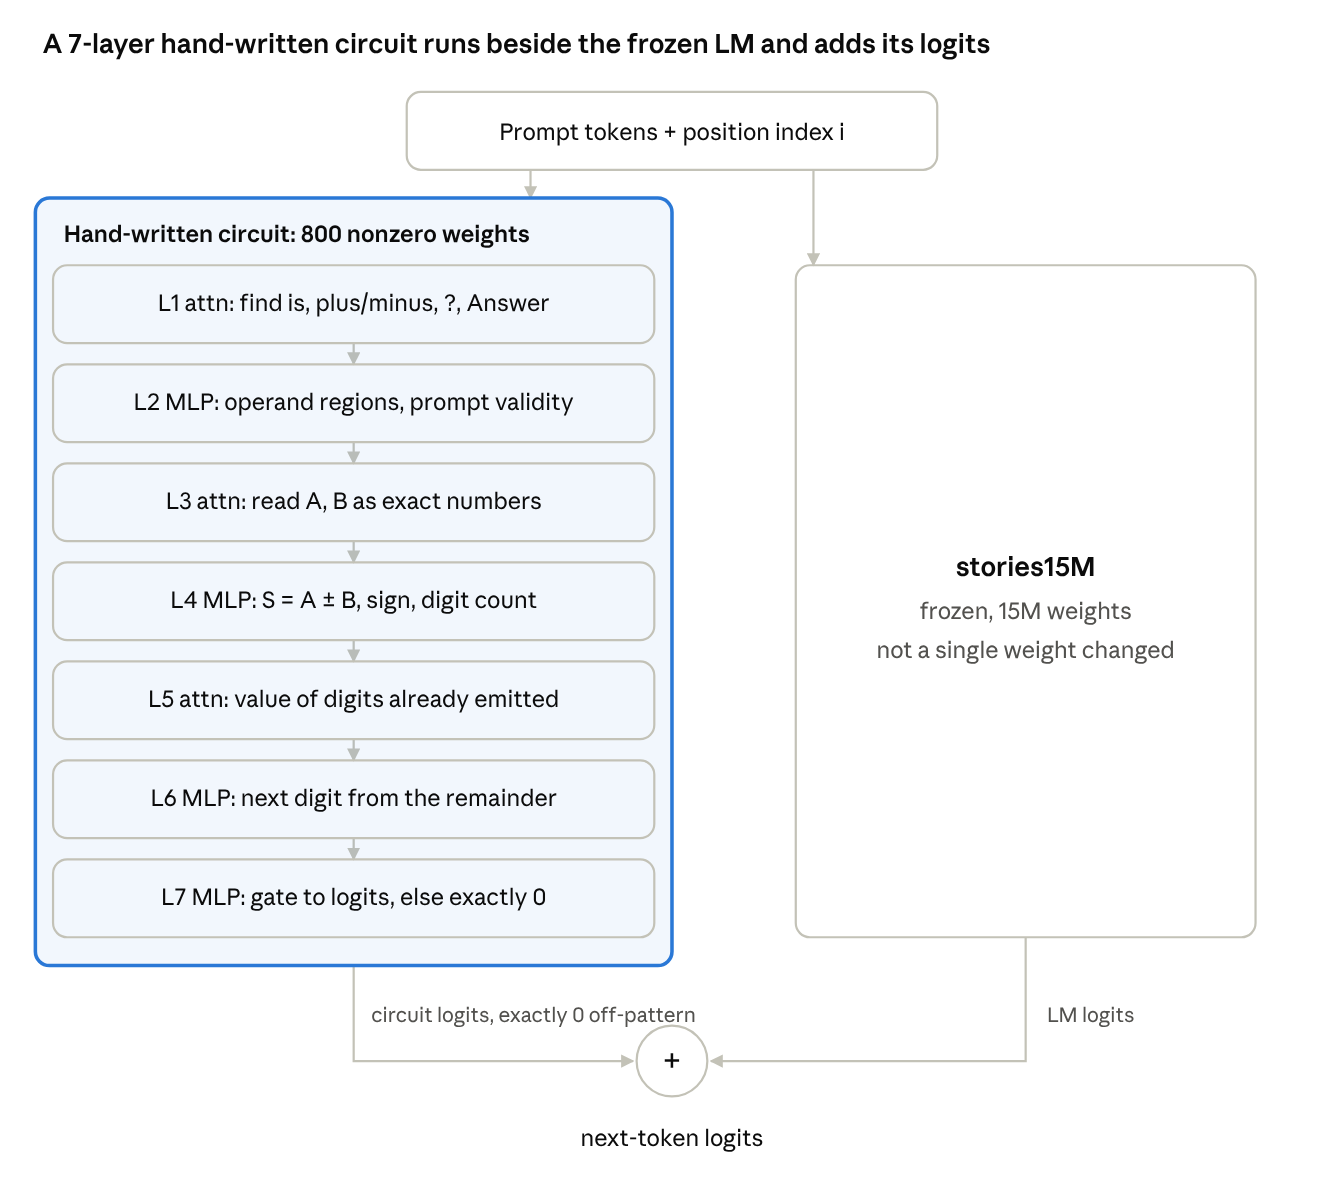
\includegraphics[width=0.82\linewidth]{fig_graft_en.png}
\caption{The grafted model: 7 hand-written layers beside the 6 frozen layers of stories15M.}
\label{fig:graft}
\end{figure}

\paragraph{How it computes.} L1 attention locates the most recent \texttt{is}, \texttt{plus}/\texttt{minus}, \texttt{?} and \texttt{Answer} tokens. L2 marks which digits belong to each operand and checks the template. L3 reads each operand as an exact number: attention weights proportional to 10 raised to each digit's significance, normalized against a fixed sink on the BOS token, return the operand's value times a known constant. L4--L6 compute $S=A\pm B$, its sign and digit count, subtract the value of digits already emitted, and select the next digit by thresholding the remainder. L7 writes large logits for the leading space or minus sign, each digit and a final newline, and outputs exactly 0 whenever the template or the stage does not match.

\begin{table}[h]
\centering
\small
\begin{tabular}{lccc}
\toprule
GPT-3 arithmetic subset & Problems & stories15M & + circuit \\
\midrule
2-digit addition / subtraction & 2{,}000 / 2{,}000 & 0.0\% / 0.0\% & 100\% / 100\% \\
3-digit addition / subtraction & 2{,}000 / 2{,}000 & 0.0\% / 0.0\% & 100\% / 100\% \\
4-digit addition / subtraction & 2{,}000 / 2{,}000 & 0.0\% / 0.0\% & 100\% / 100\% \\
5-digit addition / subtraction & 2{,}000 / 2{,}000 & 0.0\% / 0.0\% & 100\% / 100\% \\
Official rows 0--99, 5-digit add / sub & 100 / 100 & 0.0\% / 0.0\% & 100\% / 100\% \\
Exhaustive: all $a,b\in[0,99]$, add and sub & 20{,}000 & -- & 100\% \\
\bottomrule
\end{tabular}
\caption{Exact match, greedy decoding, zero-shot. Each 2{,}000-problem subset gives a 95\% Clopper--Pearson lower bound of 99.82\%. The 16{,}000 problems were regenerated following the GPT-3 sampling scheme (operands uniform below $10^N$, fixed seeds); the official rows were fetched from EleutherAI/arithmetic.}
\end{table}

\paragraph{No side effects.} On TinyStories validation text the circuit's logits are exactly zero at every position, and the loss is identical (perplexity 3.003201 with and without the graft). Greedy generations from near-miss prompts such as ``What is 3 plus 2? He did not know.'' are identical token for token. After answering, the LM continues its own text: for ``What is 7 minus 66?'' the base model writes ``Mommy, what is that?'', while the grafted model writes `` -59'' and a newline, then resumes.

\paragraph{Beyond the benchmark.} The circuit stays exact on random problems with 6, 8, 10 and 12 digits (40 per setting, addition and subtraction). It fails at 13 digits by design, because its power-of-ten table stops at $10^{12}$.

\section{In-weight surgery I: making rare tokens visible and writing new facts}\label{sec:facts}
Editing only weights the model already has, we teach it the capitals of seven countries it has never heard of. It answers correctly on up to 91\% of held-out paraphrases, from 0\%.

\paragraph{Diagnosis: rare tokens are invisible.} Before writing any fact we read the relevant embeddings. Six of the seven country tokens (Spain, Italy, Japan, Germany, England, Russia) and the token ``capital'' have pairwise cosine similarity between 0.96 and 0.999; the seven capital-city tokens are at least 0.93 similar. These tokens never occurred in training, so their embeddings drifted together. To the model, ``Spain'' and ``Japan'' are the same word, and no later edit can attach different facts to them. The first step of surgery is therefore to make them distinguishable.

\paragraph{Surgery.}
\begin{enumerate}[leftmargin=*]
\item \textbf{Tags.} A small component (norm 0.25) is added to 15 embedding rows (7 countries, ``capital'', 7 capitals), each in a direction chosen to be quiet at the model's input and output. Because embeddings are tied, a large tag would also change output logits; tags and detectors together change story loss by about 0.2\%.
\item \textbf{Detectors.} 8 low-use neurons of the layer-3 MLP detect a country or ``capital'' tag at the token itself and write a larger flag there.
\item \textbf{Dedicated attention channels.} In heads L4H3 and L4H4 we clear the low-frequency RoPE pair (44,\,45), which costs 0.6\% story loss, and reuse it so that L4H3 attends to country flags and L4H4 to the ``capital'' flag, carrying both to the answer position.
\item \textbf{AND neurons.} 7 neurons of the layer-4 MLP fire when the country flag, the capital-question flag and an answer-slot signal coincide, and write the capital through a discriminant direction over the vocabulary.
\end{enumerate}

\begin{table}[h]
\centering
\small
\setlength{\tabcolsep}{4pt}\begin{tabular}{lccccc}
\toprule
Version & Design & Held-out & Untaught country & No capital question & Story loss \\
\midrule
stories15M & 0\% & 0\% & 0\% & 0\% & 1.0997 \\
(a) Additive AND & 100\% & \textbf{91.4\%} & 65\% & 86\% & 1.1442 (+4.0\%) \\
(b) + orthogonal channels & 100\% & 80.0\% & \textbf{0\%} & 33\% & 1.1917 (+8.4\%) \\
(c) + answer-slot gating & 100\% & 68.6\% & \textbf{0\%} & \textbf{4.8\%} & 1.1703 (+6.4\%) \\
\bottomrule
\end{tabular}
\caption{Facts written into the model's own weights. ``Untaught country'': a taught capital is produced for one of 5 untaught countries. ``No capital question'': a capital is produced in prompts that mention the country but do not ask for its capital. Design: 3 templates used to set directions; held-out: 5 paraphrases never seen while writing weights.}
\end{table}

The versions trade recall for precision. The strictest one never invents a capital for an untaught country and answers without being asked in only 1 of 21 prompts, at the cost of failing paraphrases whose answer slot differs from the design templates (``\ldots is called''). All three rows are reproduced by \texttt{facts7.py} with \texttt{variant} set to a, b or c. Typical outputs: ``The capital of France is'' $\to$ `` Paris''; ``In Italy, the capital city is'' $\to$ `` Rome''.

\section{In-weight surgery II: angle-coded arithmetic}\label{sec:arith}
Again editing only existing weights, we teach the model to add two single digits. On held-out templates its exact answers rise from 6\% to 28\% overall and from 12\% to 52\% for sums up to 9.

\paragraph{The obstacle: normalization.} RMSNorm rescales every position by a factor that depends on context, so a number stored as a magnitude is distorted, and an attention head splits its weight unevenly between two digits. Both break arithmetic.

\paragraph{Angle code.} We store digit $d$ as a vector of constant norm,
\begin{equation}
v_d = K\,(\cos d\phi,\ \sin d\phi,\ 1), \qquad \phi=\pi/24,
\end{equation}
as RoPE does for positions. Normalization cannot distort it, the third component gives every digit the same attention key, and the average of $v_a$ and $v_b$ points at angle exactly $(a+b)\phi/2$. Reading the sum then needs only half-plane tests $Y\cos\beta - X\sin\beta \ge 0$, which are homogeneous and therefore insensitive to scale.

\paragraph{Surgery.}
\begin{enumerate}[leftmargin=*]
\item 20 layer-0 neurons detect each digit and write a small one-hot tag.
\item 20 layer-4 neurons re-detect the tag and write the large angle vector, so the large signal exists only between layers 4 and 5.
\item Head L5H5, the cheapest head of the last layer to remove (+0.9\% story loss when zeroed), is repurposed entirely. It attends only to digits, equally, and to a sink on the BOS token when there are none; outputs are chosen so the sink contributes almost nothing.
\item In the layer-5 MLP, 3 neurons cancel the large vector at the digit's own position (their three output gains are scalars calibrated on design digit occurrences), and 38 neurons implement 18 half-plane tests on the angle plus one presence test, which together select the answer digit, gated by the answer slot.
\end{enumerate}

The repurposed head computes the angle accurately: in a diagnostic variant of the circuit, the sum read directly from its output on design prompts was 6.95 for 3+4, 18.00 for 9+9 and 2.22 for 2+0.

\begin{table}[h]
\centering
\begin{tabular}{lcc}
\toprule
40 random digit pairs & stories15M & Edited \\
\midrule
Exact answer, design templates & 7.5\% & \textbf{33.3\%} \\
Exact answer, 4 held-out templates & 6.3\% & \textbf{27.5\%} \\
Exact answer, held-out, sums $\le 9$ & 11.9\% & \textbf{52.4\%} \\
First token, held-out & 14.4\% & 73.1\% \\
Story loss & 1.0997 & 1.1603 (+5.5\%) \\
\bottomrule
\end{tabular}
\caption{Single-digit addition written into the model's own weights.}
\end{table}

First-token accuracy overstates success because the first token of any sum from 10 to 18 is ``1''; exact answers are the honest measure. The main losses occur after the head: the final MLP must read the angle from a position that also carries other signals, and for two-digit sums it does not yet produce the second digit.

\section{A toolkit for hand-written weights}\label{sec:toolkit}
Most failed attempts in this work had the same few causes. The techniques in Table~\ref{tab:toolkit} are what fixed them, and we expect them to transfer to other models.

\begin{table}[h]
\centering
\small
\begin{tabular}{p{0.19\linewidth}p{0.32\linewidth}p{0.39\linewidth}}
\toprule
Technique & Problem it solves & How \\
\midrule
Read before writing & Edits fail silently when the model cannot represent the inputs & Check that the tokens involved have distinguishable embeddings; repair with small tags if not \\
Quiet directions & New signals interfere with what the model already does & Write into directions with low second moment at the reading layer and low energy in the output logits \\
Constant-norm codes & RMSNorm rescales magnitudes per position & Encode values as angles on a circle plus a constant presence component \\
Homogeneous tests & Thresholds drift with the normalization scale & Compare two readouts with each other (half-plane tests) instead of with a constant \\
Single-layer flags & Large signals corrupt every layer they pass through & Write a small tag early, amplify it just before the reading layer, cancel it right after \\
Dedicated attention channels & Natural attention does not look where the circuit needs & Clear a low-frequency RoPE pair in one head ($\approx$0.6\% cost) and use it for a content-only score \\
Attention sinks & A new head writes noise when its targets are absent & Give BOS a smaller fixed score and choose value directions in which BOS is zero \\
Bias substitutes & Llama layers have no biases & Use a direction whose projection is nearly constant across tokens ($\pm$6\%), computed as $\Sigma^{-1}\mu$ \\
Clipped steps & SiLU leaks below zero and grows without bound & Pair two neurons, $\mathrm{silu}(sx)-\mathrm{silu}(sx-10)$, for an output in $[0,10]$ \\
\bottomrule
\end{tabular}
\caption{Techniques that made hand-written weights work under RMS normalization.}
\label{tab:toolkit}
\end{table}

\section{Related work}
\paragraph{Weight-space programming.} Takehi et al.\ \cite{takehi2026} introduced the term for a general-purpose LLM reading and writing network weights directly. They identify what small networks were trained on, repair a failing control policy, write game-playing policies from scratch, and edit 0.016\% of Qwen3.5-0.8B's weights to remove a repetition loop, raising MATH-500 from 7.9\% to 48.1\%. They found no comparable gain on Gemma 3 270M and suggested that weight edits remove obstacles rather than add abilities. Our work is a direct follow-up on that open question, on narrower capabilities and a smaller model.

\paragraph{Compiled and hand-coded transformers.} Tracr \cite{tracr} compiles RASP programs \cite{rasp} into transformer weights; AdderBoard \cite{adderboard} collects hand-coded transformers that add 10-digit numbers with as few as 5 parameters. These build standalone networks; we write circuits that live inside or beside a pretrained model and must coexist with it.

\paragraph{Model editing.} ROME \cite{rome} and related methods change specific facts by closed-form updates to MLP weights, typically facts the model can already represent. Our facts are about tokens the model cannot initially distinguish, and our arithmetic edit adds an algorithm rather than an association.

\paragraph{Arithmetic in transformers.} Position coupling \cite{cho2024} and Abacus embeddings \cite{mcleish2024} help trained transformers generalize arithmetic to longer inputs. Our angle code is related in spirit to rotary position embeddings, applied to values instead of positions.

\section{Limitations and next steps}
\begin{itemize}[leftmargin=*]
\item \textbf{Narrow capabilities, one small model.} Seven facts, single-digit addition and benchmark-template arithmetic in a 15M-parameter model. Whether the methods scale to larger models and broader skills is open.
\item \textbf{The graft adds weights.} Section~\ref{sec:graft} widens the model with a separate block; Sections~\ref{sec:facts}--\ref{sec:arith} show the in-weight version of the idea, with lower accuracy.
\item \textbf{Template dependence.} The graft reads one prompt template; the in-weight fact edit fails on answer slots unlike those in the design templates.
\item \textbf{Side effects of in-weight arithmetic.} After writing a number, the edited model sometimes continues with further digits, and in stories that contain numbers it can insert a digit where none belongs. Story loss (+5.5\%) does not capture this, because the evaluation stories contain no numbers. A variant with a dedicated answer-slot flag removes these leaks, but we have not yet recovered its accuracy.
\item \textbf{One author, one session.} All weights were written by a single LLM in one working session, with access to forward passes. We have not measured how reliably other sessions or other LLMs reach the same results.
\item \textbf{Measured directions.} Many directions are class means and covariances from forward passes on design templates. They are closed-form statistics rather than trained parameters, but they use data.
\end{itemize}
\paragraph{Next steps.} Remove the arithmetic side effects and produce two-digit sums; scale the fact edit to dozens of facts and several relations; repeat on a larger model (stories42M, stories110M); and measure reliability across independent author sessions.

\section*{Reproducibility}\sloppy
All scripts run on CPU in minutes with fixed seeds. Graft: \texttt{llama.py}, \texttt{circuit.py}, \texttt{eval.py}, \texttt{exhaustive\_graft.py}, \texttt{preserve.py}. Facts: \texttt{surgery.py}, \texttt{facts6.py}, \texttt{facts7.py} (variants a, b, c). Arithmetic: \texttt{arith2.py}, \texttt{arith4.py}. stories15M weights from the copy of Karpathy's checkpoint in \url{https://github.com/cgbur/llama2.zig}; benchmark rows from \url{https://hf.co/datasets/EleutherAI/arithmetic}; validation stories from \url{https://hf.co/datasets/roneneldan/TinyStories}.

\begin{thebibliography}{10}
\bibitem{takehi2026} R.~Takehi, J.~Teoh, A.~Zhang, O.~Khattab. Sparks of Weight-Space Programming: LLMs can natively read \& write neural network weights. MIT CSAIL blog, 2 Nov 2026. \url{https://rikiyat.github.io/blog/weight-space-programming/}
\bibitem{gpt3} T.~Brown et al. Language Models are Few-Shot Learners. arXiv:2005.14165, 2020.
\bibitem{tinystories} R.~Eldan, Y.~Li. TinyStories: How Small Can Language Models Be and Still Speak Coherent English? arXiv:2305.07759, 2023.
\bibitem{llama2c} A.~Karpathy. llama2.c. \url{https://github.com/karpathy/llama2.c}
\bibitem{tracr} D.~Lindner et al. Tracr: Compiled Transformers as a Laboratory for Interpretability. arXiv:2301.05062, 2023.
\bibitem{rasp} G.~Weiss, Y.~Goldberg, E.~Yahav. Thinking Like Transformers. arXiv:2106.06981, 2021.
\bibitem{adderboard} AdderBoard. \url{https://github.com/anadim/AdderBoard}
\bibitem{rome} K.~Meng et al. Locating and Editing Factual Associations in GPT. arXiv:2202.05262, 2022.
\bibitem{cho2024} H.~Cho et al. Position Coupling: Improving Length Generalization of Arithmetic Transformers Using Task Structure. NeurIPS 2024. arXiv:2405.20671.
\bibitem{mcleish2024} S.~McLeish et al. Transformers Can Do Arithmetic with the Right Embeddings. NeurIPS 2024. arXiv:2405.17399.
\end{thebibliography}
\end{document}
